% siminos/cgang/flotsam.tex    master file: main.tex
% $Author$ $Date$

\section{Flotsam}
\label{s:flotsam}

\noindent
{\bf [2012-04-26 Predrag]}
\\
How to use this section? When you remove cogent text from the article
proper - clip  it and paste it into here, for possible reuse later.
\\\\\\

ES2014-05-27: Dropped this from intro: the reconstruction equations
developed in \refref{rowley_reconstruction_2000} and formulated them using a `rescaled
time' variable. Replaced with: Later on, Rowley \etal~\rf{rowley_reduction_2003} 
generalized the method in order to handle self-similar solutions. -- Consider returning
to intro if we talk about rescaled time in more detail.



The basic equivariants include
\beq
  \{{z}_1\,,\overline{z}_1 {z}_2 \}
            \,,\qquad
  \{{z}_2 \,, z_1 \overline{z}_2\}
\,.
%\label{Dang86(1.3)PK}
\eeq
We have equations \refeq{eq:DangSO2} for $\{{z}_1\,,\overline{z}_1\,,
{z}_2\,,\overline{z}_2 \}$ but perhaps need equations for the
equivariants \refeq{Dang86(1.3)PK} - have not thought this through.
[ChaosBook.org says:]

%[2013-10-07 Burak]
Differential operators acting on functions defined on a periodic domain
usually diagonalized by representing the solution as a Fourier expansion.

%[2013-10-30 Burak] cut from 2modes.tex :
\PC{notation for the translation group?}
As at least 3 dimensions are required for a continuous time flow to
exhibit chaos, in this case the \statesp\ of a $\Group$-equivariant flow
has to be at least 4\dmn. Under linear actions of $\SOn{2}$ the \statesp\
decomposes into 2\dmn\ irreducible subspaces (Fourier components) labeled
by integers $m = 0,1,2,\cdots$, which thus form the natural basis in which
to study $\SOn{2}$-equivariant flows. Nonlinear flows, such as the
1 spatial dimension \KS\ PDE for a `flame front velocity' field
$u=u(x,t)$ on a periodic domain $u(x,t) = u(x+L,t)$, given by
\beq
  u_t = F(u) = -{\textstyle\frac{1}{2}}(u^2)_x-u_{xx}-u_{xxxx}
    \,,\qquad   x \in [-L/2,L/2]
    \,,
\ee{BBks1}
can be
expressed in terms of complex Fourier coefficients $a_k(t)$,
\beq
  u(x,t)=\sum_{k=-\infty}^{+\infty} a_k (t) e^{ i q_k x}
\,,\qquad
  q_k = 2\pi k/L
\,,
\ee{BBeq:ksexp1}
as
\beq
\dot{a}_k= \pVeloc_k(a)
     = ( q_k^2 - q_k^4 )\, a_k
    - i \frac{q_k}{2} \sum_{m=-\infty}^{+\infty} a_m a_{k-m}
\,.
\ee{2m:expan}
($t \geq 0$ is the time, $x$ is the spatial coordinate, subscripts $x$
and $t$ denote partial derivatives with respect to $x$ and $t$).
Nonlinear terms mix an infinity of
Fourier components. In practice, they are represented by truncations to
a finite number of Fourier modes; the most radical truncation that
still might capture some qualitative features of a chaotic flow is to keep
only a pair of Fourier modes.


%[2013-11-06 Burak] cut from 2modes.tex :
\bea
  w  &=& - \frac{2\,u}{c_1}\,A_1 = - \frac{2\,v}{c_2}\,A_2
\continue
        &\to&\quad 2\,A_1+ A_2 = - \frac{ w}{2\,u\,v}\left(c_2\,u+2\,c_1\,v\right)
\continue
  q  &=& \frac{1}{-2e_1+e_2}
     \left(- {w^2}/{2\,u\,v} + \,2u\right)\left(c_2\,u+2\,c_1\,v\right)
%\label{PKinvEqs4}
\\
  w  &=& -\frac{1}{-2e_1+e_2} (2\,A_1+ A_2)\,q
     \,,\quad\to\quad
  q = \frac{2(-2e_1+\,e_2)\,u\,v}{c_2\,u+2\,c_1\,v}
  \,,
\nnu
\eea

%[2013-11-06 Burak] cut from 2modes.tex :
and thus we obtain \textbf{our main result}, two (bivariate)  polynomials
in two variables $\{u,v\}$ with constant coefficients
\bea
f(u,v) &=&
  c_2\,u\,(\mu_1+a_1\,u+b_1\,v)
     -
  c_1\,v\,(\mu_2+a_2\,u+b_2\,v) = 0 %Double checked DB 04-30-2012
\,,\qquad  deg(f) = 2
\continue
g(u,v) &=&
 \left(w^2 - 4\,u^2 v\right)\left(c_2\,u+2\,c_1\,v\right)^2 %Double checked DB 04-30-2012
 +\,4\,(-2e_1+e_2)^2\,u^2\,v^2 = 0
\,,\qquad  deg(g) = 6
\,,
%\label{PKinvEqs5}
\eea

%[2013-11-08 Burak] cut from 2modes.tex :

where $w$ is defined by the first equation in
\refeq{PKinvEqs4}.

Lots of coefficients, but we can
absorb some into rescaled quantities
$\tilde{u} = c_2\,u$,
$\tilde{v} = c_1\,v$,
$\tilde{a_1} = a_1/c_2$,
$\tilde{b_1} = b_1/c_1$,
$\tilde{a_2} = a_2/c_2$,
$\tilde{b_2} = b_2/c_1$,
and by using $A_1$ expression for $w$ factored out the pair of $u=0$
roots:

so we are down to 8 coefficients. Note that $e_2 \in \reals_{+}$, and if
we agree that  $\mu_1 > -\mu_2 > 0$ we can rescale the first equation so
that in new time units $\tilde{\mu}_1 =1$, $\tilde{\mu}_2 = \mu_2/\mu_1
\in \reals_{-}$, so there are 7 coefficients in all. I see no further
rescaling simplification.

As we already know $[0,0,0,0]$ and $[0,v,0,0]$ roots, one should divide
them out, and that is what we have done. Finding
roots of bivariate polynomials is not easy.

{\bf[2014-05-06 Burak]} I'll try to rewrite the abstract from the beginning,
here is its current version:
\newline
Dangelmayr\rf{Dang86} and Porter~\&\ Knobloch\rf{PoKno05} have
introduced a family of 2-Fourier mode \SOn{2}-equivariant ODEs  in order to
study bifurcations of solutions of dynamical systems in presence of
symmetries. A 4\dmn\ system of this kind is perhaps the simplest
example of a system with a continuous symmetry that can exhibit chaos, so
we use it to illustrate the role symmetries play in chaotic dynamics. We
show that a continuous symmetry induces drifts in the full
{\statesp} dynamics, drifts which obscure the chaotic dynamics. Change of
equations of motions to a {\comovframe} frame
does not eliminate these drifts: that is only attained by a
\emph{symmetry reduction} - reformulation of dynamics in a 3-dimensional
symmetry-reduced {\statesp}, where every group orbit (set of all points
reached by actions of the group of all symmetries of the equations of
motion) is replaced by a point. {\twoMode} system is a
particularly nice illustration of how this works, as in 3 dimensions we
are able to visualize everything.

We compare three symmetry reduction methods: polar coordinates, invariant
polynomial bases, and the `{\mslices}'. An invariant polynomial
basis is convenient for determination of all relative equilibria of such
system. Our conclusion, however, is that the most insight is offered by
the {\mslices}. While in general a number of local slices are
needed to cover a strange attractor\rf{atlas12}, for the {\twomode}
system there we define a unique slice hyperplane that captures
\emph{all} symmetry-reduced dynamics. \BBedit{I think this is misleading
since we have shown that single slice treatment works fine for \KS }

A Poincar\'e return map within the
slice hyperplane enables us to reduce the dynamics further, essentially
to a unimodal map, and determine, in principle, all relative periodic
orbits of the system. We can visualize each step of this process without
having to project solutions onto a submanifold since the slice hyperplane
for this system is three dimensional.

{\bf[2014-05-06 Burak]} Previously was in introduction, later commented
out:
\newline
Over the last decade, new insights into the dynamics of  [blah blah]

Our goals here are two-fold:
    \PC{{\bf[2013-10-07]} Burak's and Daniels outline of Das Artikel is
in \reffig{fig:131007outline}.
}
(i)  Illustrate \mslices\ in the lowest\dmn\ setting possible.
(ii) [blah blah].

As a motivation, consider the chaotic dynamics exhibited by the
small-cell \KS\ system studied in \refref{lanCvit07}. Examination of
typical long-time simulations shows that the spatio-temporal chaos arises
from visits to two kinds of unstable patterns, a `central wobble' region
$S_C$, and a symmetric pair of right/left `drifts' $\{S_L,S_R\}$. In
\statesp\ projections orbits stay in one neighborhood for a while, then
hop to another neighborhood, as illustrated in \reffig{f:antlong}. The
strange attractor that they explore is curved and folded in such a way
that a single local linear chart cannot cover the whole attractor,
several charts are needed, as illustrated by \reffig{fig:2ModeAtlas}\,(d).

The \statesp s of \KS\ and fluid-dynamical flows are high\dmn\ and
difficult to visualize, so here we shall illustrate the key ideas by a
much simpler example, the $\SOn{2}$-equivariant  \twoMode\ system.

%%%%%%%%%%%%%%%%%%%%%%%%%%%%%%%%%%%%%%%%%%%%%%%%%%%%%%%%%%%%
\begin{figure} %[tbp] %[h]
    \centering
 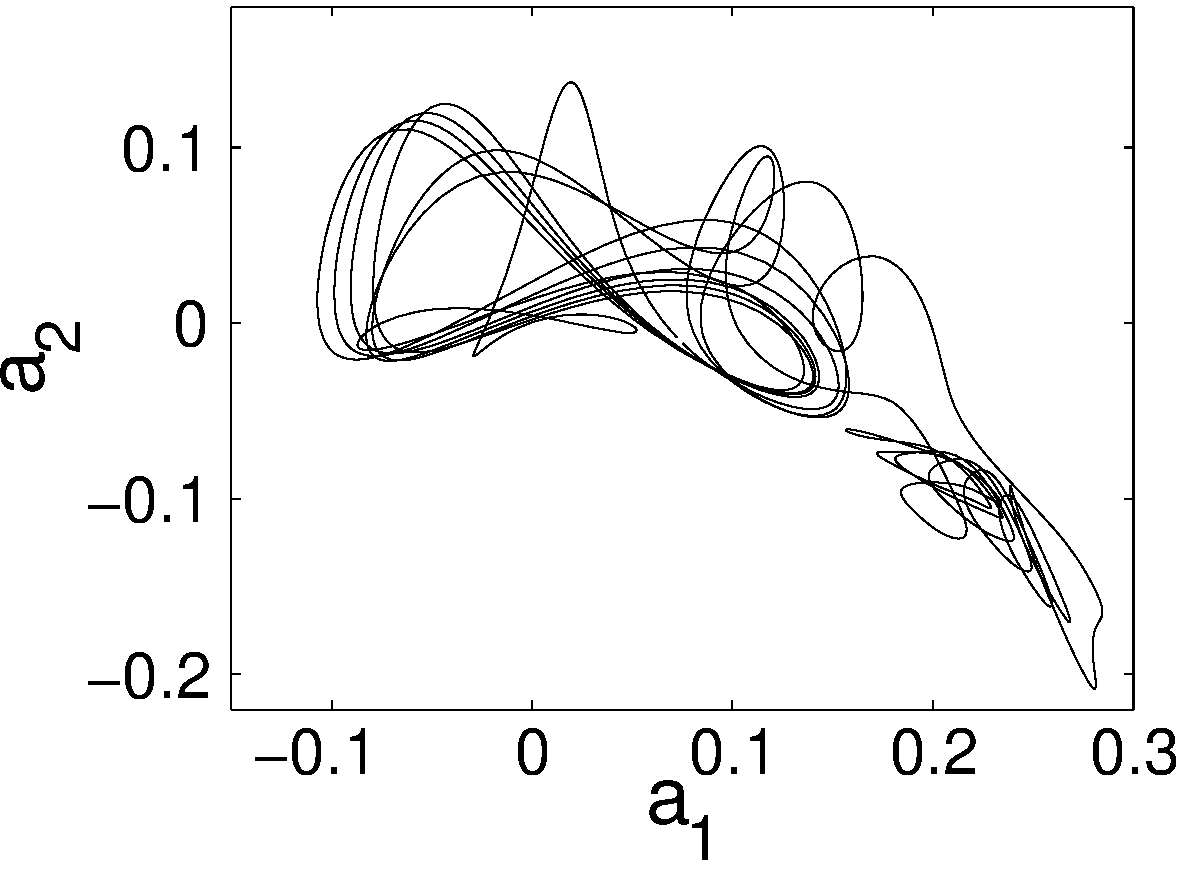
\includegraphics[width=0.40\textwidth]{kslong12}
\caption[]{
A long \KS\ \po\ of period $\period{}=355.34$ that connects
neighborhoods called `$S_C$' and `$S_R$',
(c) $[a_1,a_2]$  projection on the first two spatial Fourier modes
(from \refref{lanCvit07}).
      }
\label{f:antlong}
\end{figure}
%%%%%%%%%%%%%%%%%%%%%%%%%%%%%%%%%%%%%%%%%%%%%%%%%%%%%%%%%%%%%%

 [blah blah]


{\bf[2014-05-06 Burak]} Previous outline items:

SO2-equivariant equations:
\bea
\dot{x}_1 &=& (\mu_1 - r_1^2 + c_1 x_2)x_1 + c_1 y_1 y_2
\continue
\dot{y}_1 &=& (\mu_1 - r_1^2 - c_1 x_2)y_1 + c_1 x_1 y_2
\continue
\dot{x}_2 &=& (1 + a_2 r_1^2)x_2 + (x_1^2 - y_1^2) + y_2
\continue
\dot{y}_2 &=& (1 + a_2 r_1^2)y_2 + 2 x_1 y_1 - x_2
\continue
		  && \mbox{where } r_1^2 = x_1^2 + y_1^2\, , \quad r_2^2 = x_2^2 + y_2^2
\,.
\label{2mode4Dset1}
\eea


%%%%%%%%%%%%%%%%%%%%%%%%%%%%%%%%%%%%%%%%%%%%%%%%%%%%%%%%%%%%%%%%%%%%%%%%%%%%%%%%%%%%%%%%%%%%%%%%%
\subsection{To do}
\label{s:ToDo}

\begin{itemize}
  \item[10.11] Visualizations of the 4-dimensional {\twoMode} system
  \item[10.1?] draw a group orbit for the {\twoMode} model
  \item[10.22] {\twoMode} system in polar coordinates (maybe skip)
  \item[10.23] The \reqva\ of the {\twoMode} system
  \item[10.24] Plotting the \reqva\ of
           the {\twoMode} system in invariant coordinates
  \item[10.25] Plotting the \reqva\ of
           the {\twoMode} system in Cartesian coordinates
           \refeq{2mode4D}
  \item[10.2?] construct a 2-chart atlas
           \reffig{fig:2ModeAtlas} for a {\twoMode} system
  \item
        compute analytically the \stabmat\ \Mvar\ in polar coordinates
  \item
        Study eigenvalues, keep playing with parameters. We would like
        -preferably- no \reqv\ to be attracting limit cycle, and several of
        the \reqva\ to be complex-pair unstable, leading to chaos, to be
        visualized and sliced in Cartesian coordinates.
  \item
        If you find a nice chaotic attractors, others can join in
        constructing an atlas for it. We just need one and only one
        example with non-trivial \chartBord s and at least 2 charts.
\end{itemize}

 [blah blah]

\begin{itemize}
  \item $\REQV{}{1} = (r_1,r_2,\psi)=(0.0516508, 1.26311,?)$ and
        $\REQV{}{2} = (0.467095,0.2146,?)$
  \item their plots in the Cartesian coordinates
  \item $\dot{\theta}$ to see how slow/fast are they. $\dot{\theta}$
        might be related to 4th eigenvalue, when you go back
        to Cartesian coordinates
  \item stability eigenvalues, eigenvectors of the \eqv\ $\EQV{0}$ at
        origin, at your parameter values - if it is stable, everything
        just might fall into it and die.
  \item plots of small perturbations of the above \eqv\ and \reqva\ in
        the Cartesian coordinates to see whether the dynamics looks
        chaotic
  \item $\REQV{}{1}$: 2 large positive eigenvalues looks scary - probably
        nothing re-visits this \reqv. A mildly unstable complex pair
        would have been sweeter. You get complex eigenvalue by Hopf-bifurcating off a
        stable orbit, typically.
  \item $\REQV{}{1}$: Does either unstable eigenvalue become a complex
        eigenvalue pair in Cartesian coordinates?
  \item $\REQV{}{2}$: contracting eigenvalues have very small imaginary
        part, so the presumably just rocket toward the \reqv, not much
        spiraling there. At least the unstable eigenvalue seems slow
        compared to all other eigenvalues.
  \item $\REQV{}{1}$: Does the unstable eigenvalue become a complex
        eigenvalue pair in Cartesian coordinates?
\end{itemize}

 [blah blah]



%%%%%%%%%%%%%%%%%%%%%%%%%%%%%%%%%%%%%%%%%%%%%%%%
 2011-09-09, 2012-03-30 Predrag: add BeThMovFr to
            continuous.tex overheads, and ChaosBook
 replace A27movFrame*.* everywhere
\begin{figure}
  	\begin{center}
(a)
(b)
(c)
(d)
    \end{center}
  \caption{
  \twoMode, $d=4 \to 3$~dimensional $\{x_1,x_2,z\}$ projections:
  (a)
  The strange attractor.
  (b)
 (c)
 In contrast
 to the 1\dmn\ \poincBord s of \reffig{fig:2modeSects}, here ...
 (d)
  }
\label{fig:2ModeAtlas}
\end{figure}
%%%%%%%%%%%%%%%%%%%%%%%%%%%%%%%%%%%%%%%%%%%%%%%%%

 [blah blah]

 [blah blah]

\section{Chart}
\label{s:slice}

 [blah blah]

One can write the equations for the flow in the \reducedsp\
$\dot{\sspRed} = \velRed(\sspRed)$ (for details see, for example,
\refref{DasBuch}) as
\bea
\velRed(\sspRed) &=& \vel(\sspRed)
     \,-\, \dot{\gSpace}(\sspRed) \, \groupTan(\sspRed)
\label{2modesEqMotMFrame}\\
\dot{\gSpace}(\sspRed) &=& \braket{\vel(\sspRed)}{\sliceTan{}}
                       /\braket{\groupTan(\sspRed)}{\sliceTan{}}
\,
\label{2modesreconstrEq}
\eea
which confines the motion to the \slice\ hyperplane. Thus, the dynamical
system $\{\pS,\map^t\}$ with continuous symmetry \Group\ is replaced by
the {\reducedsp} dynamics $\{\pSRed,\mapRed^t\}$: The velocity in the
full \statesp\ $\vel$ is the sum of $\velRed$, the velocity component in
the \slice\ hyperplane, and $\dot{\gSpace}\,\groupTan$, the velocity
component along the group tangent space. The integral of the {\em
reconstruction equation} for $\dot{\gSpace}$ keeps track of the group
shift in the full \statesp.


 [blah blah]

{\bf[2014-05-07 Burak]} Taken out from \refsect{s-slice}:
\newline

\refFig{fig:BBgorbitsandslice} shows a 3D projection of the 4D \statesp\ corresponding
to an $m=2$ truncation of \refeq{FourierSeries}, for which \refeq{mmodeLieEl} and \refeq{mmodeLg}
are $4 \times 4$ matrices. The \slicePlane\ defined by \refeq{firstmodetemp}, three
different group orbits and the group tangents evaluated at their intersections with the \slicePlane\
are visualized in \reffig{fig:BBgorbitsandslice}. One can see as the magnitude of the second mode (the vertical axis)
relative to the first mode increases, the group tangent gets closer to being
parallel to the \slicePlane , however, it still has a non zero perpendicular component. The vertical
axis ($x_2$) in \reffig{fig:BBgorbitsandslice} lies on the \sliceBord\ of the
\slicePlane .
